\begin{enunciado}{\ejExtra}
  \begin{enumerate}[label=(\alph*)]
    \item
          Sean $L_1 = \set{(x,y,z) \en \reales^3 : x = y,\ z = 0}$ y
          $L_2 = \set{(x,y,z) \en \reales^3 : x = y = z }$. Describir $S = L_1 + L_2$ y dar una base ortonormal para dicho subespacio.

    \item
          Sea $P \en \reales^{3 \times 3}$ el proyector ortogonal a $S$. A partir de $P(0, -2, 5)$ calcular la distancia de
          $(0, -2, 5)$ a $S$.

    \item Sea
          $Q
            =
            \matriz{ccc}{
              0 & -1 & 0 \\
              1 & 0 & 0 \\
              0 & 0 & 1
            }.
          $
          Probar que $(QP)^tQ = P$.
  \end{enumerate}
\end{enunciado}

\begin{enumerate}[label=(\alph*)]
  \item Los subespacios $L_1$ y $L_2$ en generadores:
        $$
          L_1 = \ket{(1,1,0)}
          \ytext
          L_2 = \ket{(1,1,1)}
        $$
        Para calcular el espacio suma $S = L_1 + L_2$, dado que son dos vectores \textit{linealmente independientes}:
        $$
          S = \set{(1,1,0), (1,1,1)}
          \quad
          \text{con la \textit{base ortonormal}}
          \quad
          BON_S = \set{(\frac{1}{\sqrt{2}}, \frac{1}{\sqrt{2}}, 0), (0,0,1)}
        $$
        La base ortonormal la podés conseguir con Gram-Schmidt. De yapa hago una \textit{base ortonormal} del complemento ortogonal de $S$, $S^\perp$:
        $$
          BON_{S^\perp} = \set{(\frac{1}{\sqrt{2}}, -\frac{1}{\sqrt{2}}, 0)}
        $$

  \item

        $$
          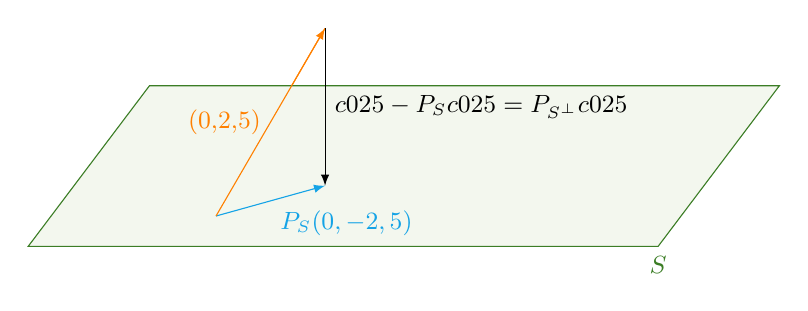
\begin{tikzpicture}[scale = 1, every node/.style={font=\small}]
            \coordinate[] (A) at (-1,0.5,0);
            \coordinate[] (B) at (-1,0,4);
            \coordinate[] (C) at (7,0,4);
            \coordinate[] (D) at (7,0.5,0);
            \coordinate[] (P) at (2,2,2);
            \coordinate[] (O) at (1,0,3);
            \coordinate[] (PP) at (2,0,2);
            \filldraw[] (O) circle[radius = 1pt] node[below]{$O$};
            \draw[orange] (O) -- (P) node[midway, left]{$(0,-2,5)$};
            \draw[OliveGreen, fill=OliveGreen!5!white] (A)--(B)--(C)node[below]{$S$}--(D)--cycle;
            \draw[thin,-latex, black] (P)--(PP) node[midway,right]{$
                \ot\matriz{c}{
                  0\\
                  2\\
                  5
                }
                -
                P_S
                \matriz{c}{
                  0\\
                  2\\
                  5
                }
                =
                P_{S^\perp}
                \matriz{c}{
                  0\\
                  2\\
                  5
                }
              $};
            \draw[thin,-latex, Cerulean] (O)--(PP) node[midway, below right]{$P_{S}(0,-2,5)$} ;
            \draw[-latex,orange] (O)--(P) node[midway, left]{(0,2,5)};
          \end{tikzpicture}
        $$
        La distancia se puede calcular como:
        $$
          \begin{array}{rcl}
            \textstyle
            d(
            \matriz{c}{
            0                   \\
            2                   \\
              5
            },
            S) =
            \norma{
              \matriz{c}{
            0                   \\
            2                   \\
                5
              }
              -
              P_S
              \matriz{c}{
            0                   \\
            2                   \\
                5
              }
            }
             & = &
            \norma{
              P_{S^\perp}
              \matriz{c}{
            0                   \\
            2                   \\
                5
              }
            }                   \\\\
             & = & \norma{
              (\frac{1}{\sqrt{2}}, -\frac{1}{\sqrt{2}}, 0)
              \accion
              \matriz{c}{
            0                   \\
            2                   \\
                5
              }
              \cdot
              \matriz{c}{
            \frac{1}{\sqrt{2}}  \\
            -\frac{1}{\sqrt{2}} \\
                0
              }
            }                   \\
             & = &
            |-\sqrt{2}|
            \norma{
              \matriz{c}{
            \frac{1}{\sqrt{2}}  \\
            -\frac{1}{\sqrt{2}} \\
                0
              }
            }                   \\
             & = &
            \sqrt{2}
          \end{array}
        $$

  \item
        Notando que:
        $$
          Q \cdot Q^t = I_3,
        $$
        sale en 2 patadas, si no lo notás, calculá el proyector ortogonal sobre el subespacio $S$, $P$, al final se explica como.
        (\hyperlink{teoria-3:proyector}{acá dice bien como \click}).
        $$
          (QP)^tQ  = P
          \sii
          (QP)^tQ\blue{Q^t}  = P\blue{Q^t}
          \sii
          (QP)^t = P\blue{Q^t}
          \sii
          P^tQ^t = P\blue{Q^t}
          \Sii{\red{!!}}
          PQ^t = P\blue{Q^t}
        $$
        $P$ es un \textit{proyector ortogonal} ¡Su expresión matricial es simétrica! $P = P^t$,
        después de todo el proyector se calcula como $P = C C^t$ donde $C$ es la matriz que tiene como columnas los
        elementos de la $BON_S$ y es evidente que si:
        $$
          P \igual{$\llamada1$} C C^t
          \Sii{transpongo}
          P^t = (C C^t)^t = (C^t)^tC^t = C C^t \igual{$\llamada1$} P
        $$
\end{enumerate}

\begin{aportes}
  \item \aporte{\dirRepo}{naD GarRaz \github}
\end{aportes}
